\mode*
\part{Input/Output}

\lecture[io]{io}{io}

\section{Principles of I/O Hardware}

\begin{frame}{I/O Hardware}
  \begin{block}{Different people, different view}
    \begin{itemize}
    \item \alert{Electrical engineers:} chips, wires, power supplies, motors...
    \item \alert{Programmers:} interface presented to the software
      \begin{itemize}
      \item the commands the hardware accepts
      \item the functions it carries out
      \item the errors that can be reported back
      \item ...
      \end{itemize}
    \end{itemize}
  \end{block}
\end{frame}

\begin{frame}{I/O Devices}
  Roughly two Categories:
  \begin{enumerate}
  \item \alert{Block devices:} store information in fix-size blocks
  \item \alert{Character devices:} deal with streams of characters
  \end{enumerate}
\end{frame}

This classification scheme is not perfect. Some devices just do not fit in.  Clocks, for
example, are not block addressable. Nor do they generate or accept character streams. All
they do is cause interrupts at well-defined intervals. Memory-mapped screens do not fit
the model well either. Still, the model of block and character devices is general enough
that it can be used as a basis for making some of the operating system software dealing
with I/O device independent. The file system, for example, deals just with abstract block
devices and leaves the device-dependent part to lower-level software\citetitle[Sec.~5.1.1,
\emph{I/O Devices}]{tanenbaum2008modern}.

\begin{frame}{Device Controllers}
  I/O units usually consist of
  \begin{enumerate}
  \item a mechanical component
  \item an electronic component is called the \emph{device controller} or \emph{adapter}
    \begin{itemize}
    \item[e.g.] video adapter, network adapter...
    \end{itemize}
  \end{enumerate}
  \begin{center}
    \mode<beamer>{
      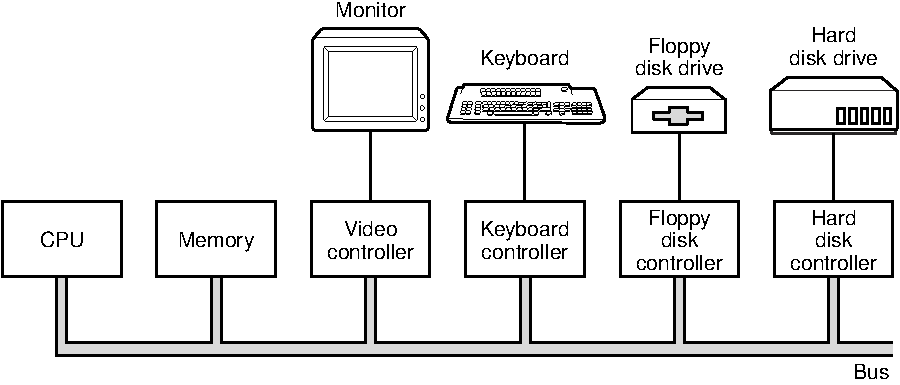
\includegraphics[width=\textwidth]{mos-figs-1-5}
    } \mode<article>{
      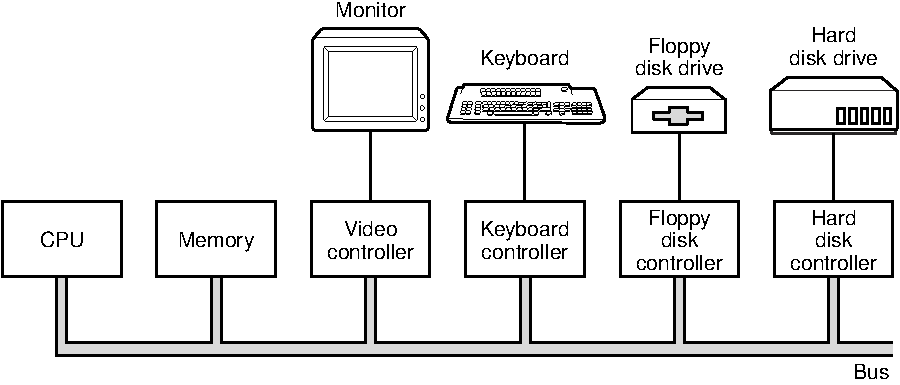
\includegraphics[width=.6\textwidth]{mos-figs-1-5}
    }
  \end{center}
\end{frame}

\begin{frame}
  \begin{description}
  \item[Port:] A connection point. A device communicates with the machine via a port ---
    for example, a serial port.
  \item[Bus:] A set of wires and a rigidly defined protocol that specifies a set of
    messages that can be sent on the wires.
  \item[Controller:] A collection of electronics that can operate a port, a bus, or a device.
    \begin{itemize}
    \item[e.g.] serial port controller, SCSI bus controller, disk controller...
    \end{itemize}
  \end{description}
\end{frame}

\begin{frame}{The Controller's Job}
  \begin{block}{Examples:}
    \begin{itemize}
    \item \alert{Disk controllers:} convert the serial bit stream into a block of bytes
      and perform any error correction necessary
    \item \alert{Monitor controllers:} read bytes containing the characters to be
      displayed from memory and generates the signals used to modulate the CRT beam to
      cause it to write on the screen
    \end{itemize}
  \end{block}
\end{frame}

The interface between the controller and the device is often a very low-level interface. A
disk, for example, might be formatted with 10,000 sectors of 512 bytes per track. What
actually comes off the drive, however, is a serial bit stream, starting with a
\emph{preamble}, then the 4096 bits in a sector, and finally a checksum, also called an
\emph{Error-Correcting Code} (\emph{ECC}). The preamble is written when the disk is
formatted and contains the cylinder and sector number, the sector size, and similar data,
as well as synchronization information\citetitle[Sec.~5.1.2, \emph{Device
  Controllers}]{tanenbaum2008modern}.

The controller's job is to convert the serial bit stream into a block of bytes and perform
any error correction necessary. The block of bytes is typically first assembled, bit by
bit, in a buffer inside the controller. After its checksum has been verified and the block
has been declared to be error free, it can then be copied to main memory.

The controller for a monitor also works as a bit serial device at an equally low level. It
reads bytes containing the characters to be displayed from memory and generates the
signals used to modulate the CRT beam to cause it to write on the screen. The controller
also generates the signals for making the CRT beam do a horizontal retrace after it has
finished a scan line, as well as the signals for making it do a vertical retrace after the
entire screen has been scanned. If it were not for the CRT controller, the operating
system programmer would have to explicitly program the analog scanning of the tube. With
the controller, the operating system initializes the controller with a few parameters,
such as the number of characters or pixels per line and number of lines per screen, and
lets the controller take care of actually driving the beam. Flat-screen TFT displays are
different, but just as complicated.

\begin{frame}{Inside The Controllers}
  \begin{description}
  \item[Control registers:] for communicating with the CPU (R/W, On/Off...)
  \item[Data buffer:] for example, a video RAM
  \end{description}
  \begin{itemize}
  \item[Q:] How the CPU communicates with the control registers and the device data
    buffers?
  \item[A:] Usually two ways...
  \end{itemize}
\end{frame}

\begin{frame}[fragile]
  \begin{itemize}
  \item[(a)] Each control register is assigned an I/O port number, then the CPU can do, for
    example,
    \begin{itemize}
    \item read in control register \texttt{PORT} and store the result in CPU register
      \texttt{REG}.\\
      \mint[fontsize=\small]{nasm}|    IN REG, PORT|
    \item write the contents of \texttt{REG} to a control register\\
      \mint[fontsize=\small]{nasm}|    OUT PORT, REG|
    \end{itemize}
    \alert{Note:} the address spaces for memory and I/O are different. For example,
    \begin{itemize}
    \item read the contents of I/O port 4 and puts it in \texttt{R0}\\
      \mint[fontsize=\small]{nasm}|     IN R0, 4 ; 4 is a port number|
    \item read the contents of memory word 4 and puts it in \texttt{R0}\\
      \mint[fontsize=\small]{nasm}|    MOV R0, 4 ; 4 is a memory address|
    \end{itemize}
  \end{itemize}
\end{frame}

\begin{frame}{Address spaces}
  \begin{center}
    \mode<beamer>{
      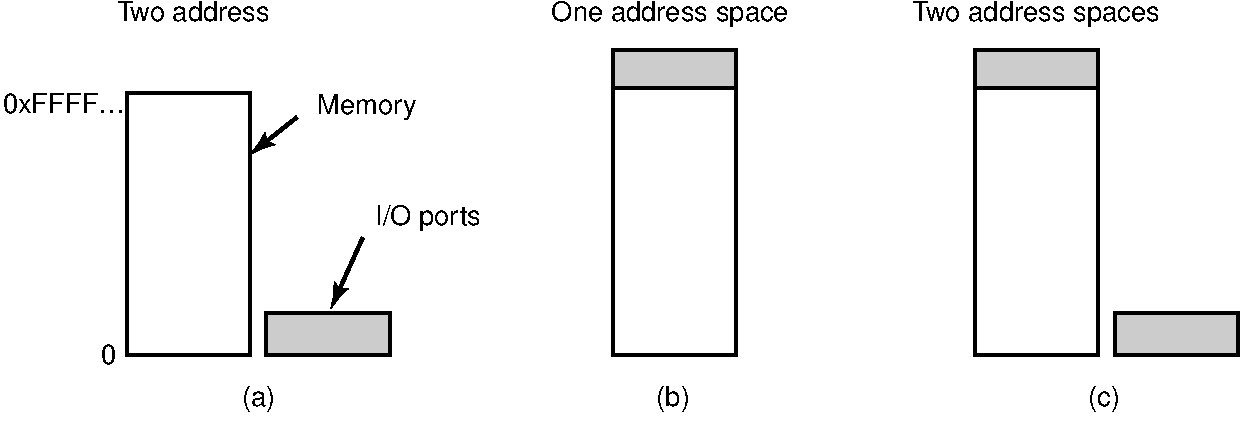
\includegraphics[width=.9\textwidth]{mos-5-2}
    } \mode<article>{
      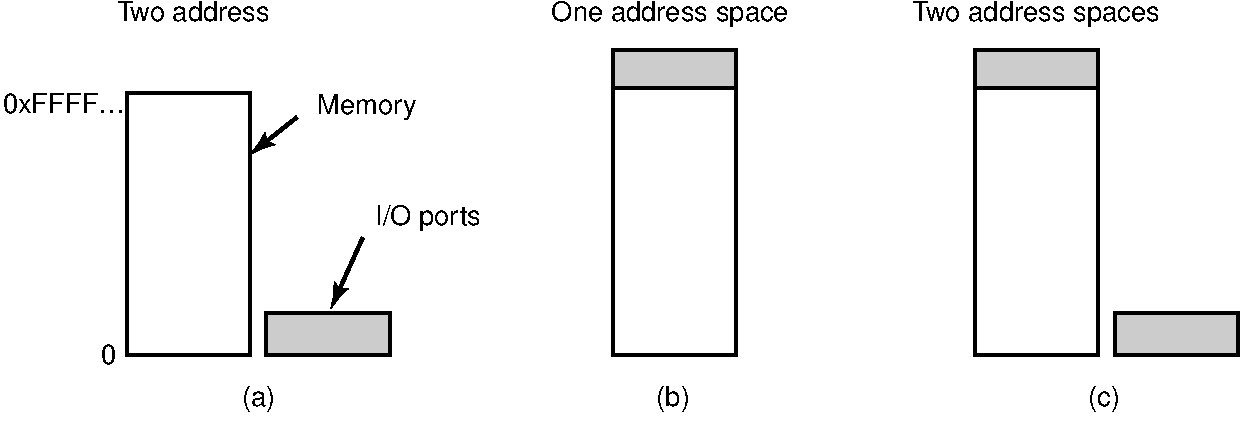
\includegraphics[width=.7\textwidth]{mos-5-2}
    }
  \end{center}
  \begin{itemize}
  \item[(a)] Separate I/O and memory space
  \item[(b)] \alert{Memory-mapped I/O:} map all the control registers into the memory
    space. Each control register is assigned a unique memory address.
  \item[(c)] \alert{Hybrid:} with memory-mapped I/O data buffers and separate I/O ports
    for the control registers. For example, Intel Pentium
    \begin{itemize}
    \item Memory addresses 640K to 1M being reserved for device data buffers
    \item I/O ports 0 through 64K.
    \end{itemize}
  \end{itemize}
\end{frame}

How can the processor give commands and data to a controller to accomplish an I/O
transfer? The short answer is that the controller has one or more registers for data and
control signals. The processor communicates with the controller by reading and writing bit
patterns in these registers. \emph{One way in which this communication can occur is through
  the use of special I/O instructions that specify the transfer of a byte or word to an
  I/O port address}. The I/O instruction triggers bus lines to select the proper device
and to move bits into or out of a device register. \emph{Alternatively, the device
  controller can support memory-mapped I/O}. In this case, the device-control registers
are mapped into the address space of the processor. The CPU executes I/O requests using
the standard data-transfer instructions to read and write the device-control registers.
Some systems use both techniques. For instance, PCs use I/O instructions\citetitle[Sec.~12.2,
\emph{I/O Hardware}]{silberschatz11essentials}.

How do these schemes work? In all cases, when the CPU wants to read a word, either from
memory or from an I/O port, it puts the address it needs on the bus' address lines and
then asserts a \texttt{READ} signal on a bus' control line. A second signal line is used to
tell whether I/O space or memory space is needed. If it is memory space, the memory
responds to the request. If it is I/0 space, the I/0 device responds to the request. If
there is only memory space [as in (b)], every memory module and every I/O device compares
the address lines to the range of addresses that it services. If the address falls in its
range, it responds to the request. Since no address is ever assigned to both memory and an
I/O device, there is no ambiguity and no conflict\citetitle[Sec.~5.1.3, \emph{Memory-mapped
  I/O}]{tanenbaum2008modern}.

\begin{frame}{Advantages of Memory-mapped I/O}
  \begin{block}{No assembly code is needed (\texttt{IN, OUT...})}
    With memory-mapped I/O, device control registers are just variables in memory and can
    be addressed in C the same way as any other variables. Thus with memory-mapped I/O, a
    I/O device driver can be written entirely in C.
  \end{block}
  \begin{block}{No special protection mechanism is needed}
    The I/O address space is part of the kernel space, thus cannot be touched directly by
    any user space process.
  \end{block}
\end{frame}

The two schemes for addressing the controllers have different strengths and
weaknesses. Let us start with the advantages of memory-mapped I/O. First, if special I/0
instructions are needed to read and write the device control registers, access to them
requires the use of assembly code since there is no way to execute an IN or OUT
instruction in C or C++. Calling such a procedure adds overhead to controlling I/O. In
contrast, with memory-mapped I/O, device control registers are just variables in memory
and can be addressed in C the same way as any other variables. Thus with memory-mapped
I/O, a I/O device driver can be written entirely in C. Without memory-mapped I/O, some
assembly code is needed\citetitle[Sec.~5.1.3, \emph{Memory-mapped I/O}]{tanenbaum2008modern}.

Second, with memory-mapped I/O, no special protection mechanism is needed to keep user
processes from performing I/O. All the operating system has to do is refrain from putting
that portion of the address space containing the control registers in any user's virtual
address space. Better yet, if each device has its control registers on a different page of
the address space, the operating system can give a user control over specific devices but
not others by simply including the desired pages in its page table. Such a scheme can
allow different device drivers to be placed in different address spaces, not only reducing
kernel size but also keeping one driver from interfering with others.

Third, with memory-mapped I/O, every instruction that can reference memory can also
reference control registers. For example, if there is an instruction, \texttt{TEST}, that
tests a memory word for 0, it can also be used to test a control register for 0, which
might be the signal that the device is idle and can accept a new command.  The assembly
language code might look like this:

\begin{nasmcode}
        LOOP: TEST   PORT_4  ;check if port 4 is 0
              BEQ    READY   ;if it is 0, go to ready
              BRANCH LOOP    ;otherwise, continue testing
        READY:    
\end{nasmcode}

If memory-mapped I/O is not present, the control register must first be read into
the CPU, then tested, requiring two instructions instead of one. In the case of the
loop given above, a fourth instruction has to be added, slightly slowing down the
responsiveness of detecting an idle device.

\begin{frame}{Disadvantages of Memory-mapped I/O}
  \begin{block}{Caching problem}
    \begin{itemize}
    \item Caching a device control register would be disastrous
    \item Selectively disabling caching adds extra complexity to both hardware and the OS
    \end{itemize}
  \end{block}
  \begin{block}{Problem with multiple buses}
    \begin{figure}[h]
      \centering
      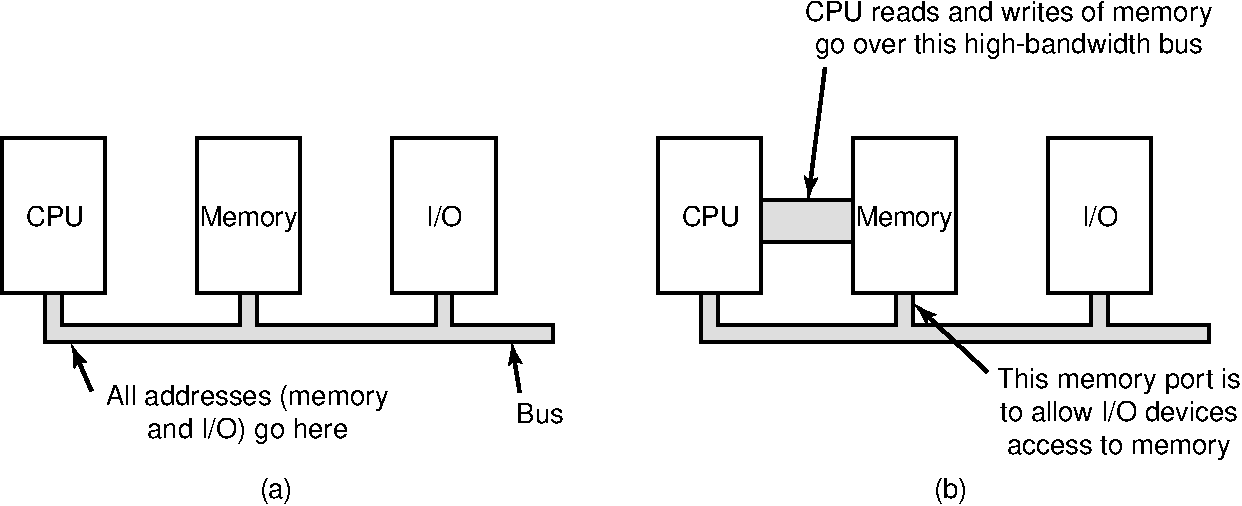
\includegraphics[width=.8\textwidth]{mos-5-3}
      \caption{(a) A single-bus architecture. (b) A dual-bus memory architecture.}
      \label{fig:mmap-bus}
    \end{figure}
  \end{block}  
\end{frame}

In computer design, practically everything involves trade-offs, and that is the case here
too. Memory-mapped I/O also has its disadvantages. First, most computers nowadays have
some form of caching of memory words. Caching a device control register would be
disastrous. Consider the assembly code loop given above in the presence of caching. The
first reference to \texttt{PORT\_4} would cause it to be cached. Subsequent references would
just take the value from the cache and not even ask the device. Then when the device
finally became ready, the software would have no way of finding out. Instead, the loop
would go on forever\citetitle[Sec.~5.1.3, \emph{Memory-mapped I/O}]{tanenbaum2008modern}.

To prevent this situation with memory-mapped I/O, the hardware has to be equipped with the
ability to selectively disable caching, for example, on a per page basis. This feature
adds extra complexity to both the hardware and the operating system, which has to manage
the selective caching.

Second, if there is only one address space, then all memory modules and all I/O devices
must examine all memory references to see which ones to respond to.  If the computer has a
single bus, as in Fig~\ref{fig:mmap-bus}(a), having everyone look at every address is
straightforward.

% \begin{figure}[h]
%   \centering
%   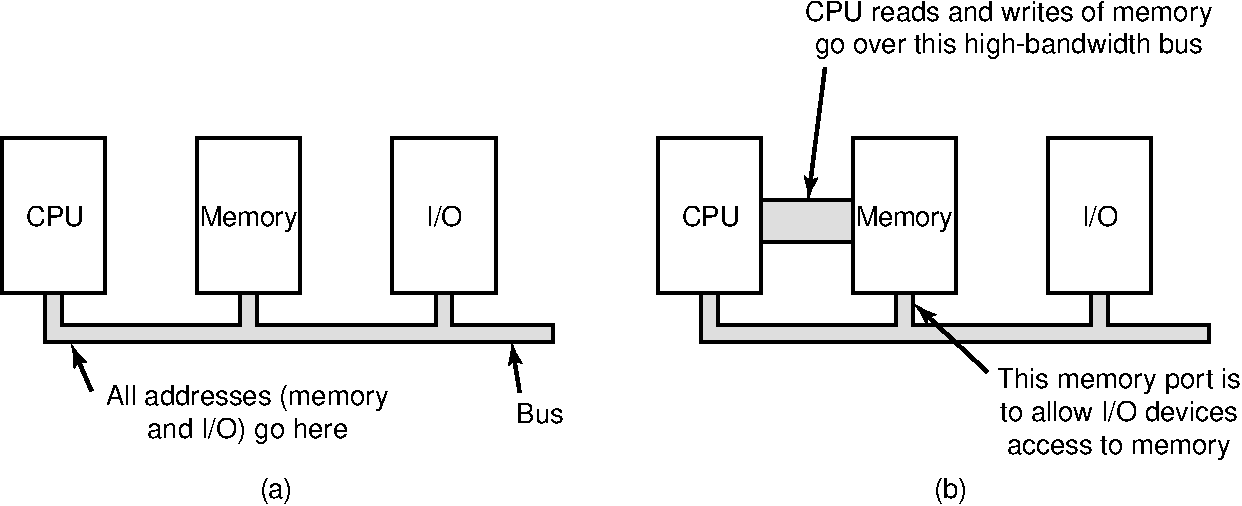
\includegraphics[width=.7\textwidth]{mos-5-3}
%   \caption{(a) A single-bus architecture. (b) A dual-bus memory architecture.}
%   \label{fig:mmap-bus}
% \end{figure}

However, the trend in modern personal computers is to have a dedicated high-speed memory
bus, as shown in Fig~\ref{fig:mmap-bus}(b), a property also found in main-frames,
incidentally. This bus is tailored to optimize memory performance, with no compromises for
the sake of slow I/O devices. Pentium systems can have multiple buses (memory, PCI, SCSI,
USB, ISA), as shown in Fig~\ref{fig:pentium-buses}.

\begin{figure}[h]
  \centering
  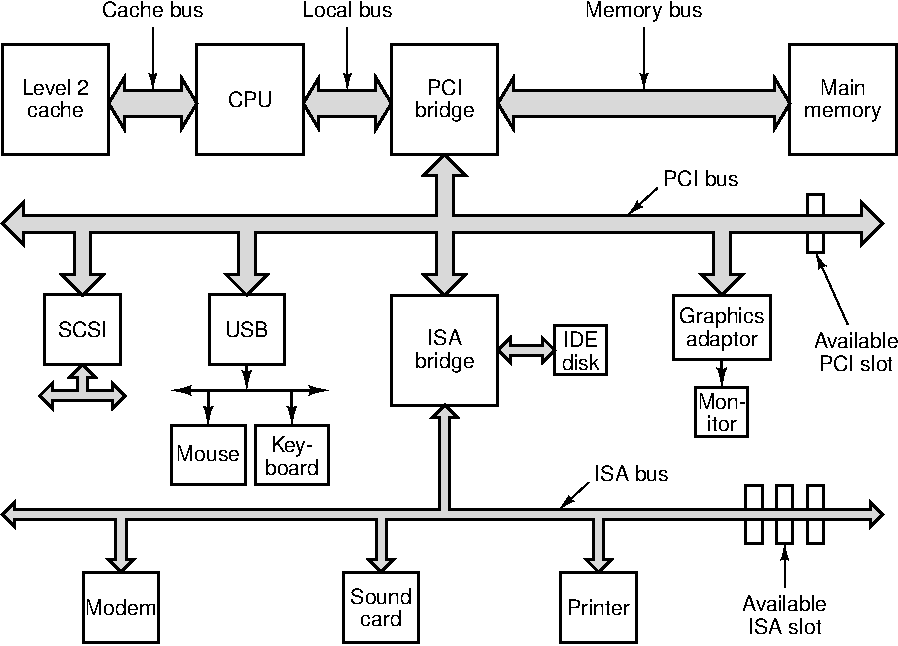
\includegraphics[width=.5\textwidth]{mos-1-11}
  \caption{The structure of a large Pentium system}
  \label{fig:pentium-buses}
\end{figure}

The trouble with having a separate memory bus on memory-mapped machines is that the I/O
devices have no way of seeing memory addresses as they go by on the memory bus, so they
have no way of responding to them. Again, special measures have to be taken to make
memory-mapped I/O work on a system with multiple buses. One possibility is to first send
all memory references to the memory. If the memory fails to respond, then the CPU tries
the other buses. This design can be made to work but requires additional hardware
complexity.

A second possible design is to put a snooping device on the memory bus to pass all
addresses presented to potentially interested I/O devices. The problem here is that I/0
devices may not be able to process requests at the speed the memory can.

A third possible design, which is the one used on the Pentium configuration of
Fig~\ref{fig:pentium-buses}, is to filter addresses in the PCI bridge chip. This chip
contains range registers that are preloaded at boot time. For example, 640K to 1M could be
marked as a nonmemory range. Addresses that fall within one of the ranges marked as
nonmemory are forwarded onto the PCI bus instead of to memory. The disadvantage of this
scheme is the need for figuring out at boot time which memory addresses are not really
memory addresses. Thus each scheme has arguments for and against it, so compromises and
trade-offs are inevitable.

\subsection{Programmed I/O}

\begin{frame}{Programmed I/O}{Handshaking}
  \begin{center}
    \mode<beamer>{
      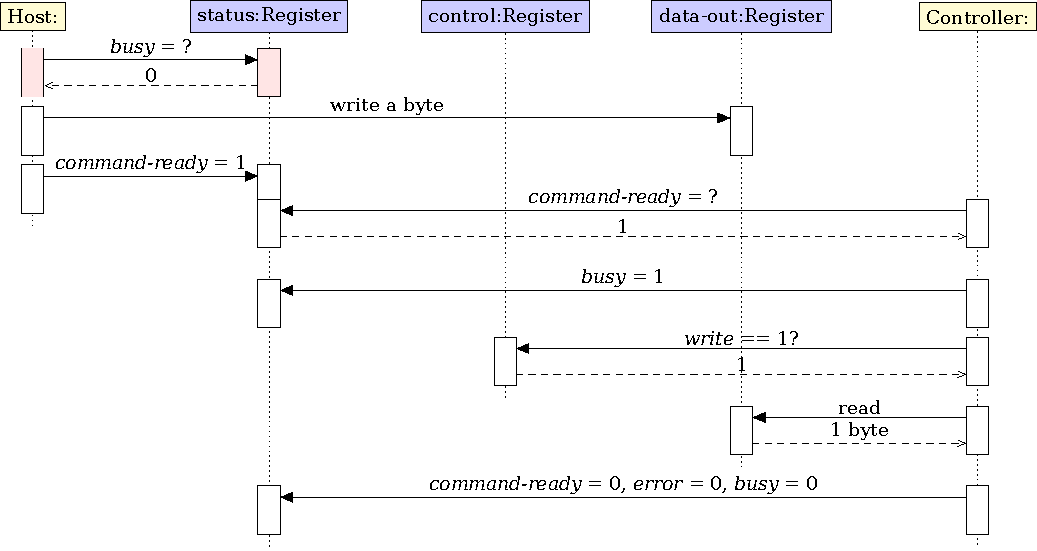
\includegraphics[width=\textwidth]{handshaking}
    } \mode<article>{
      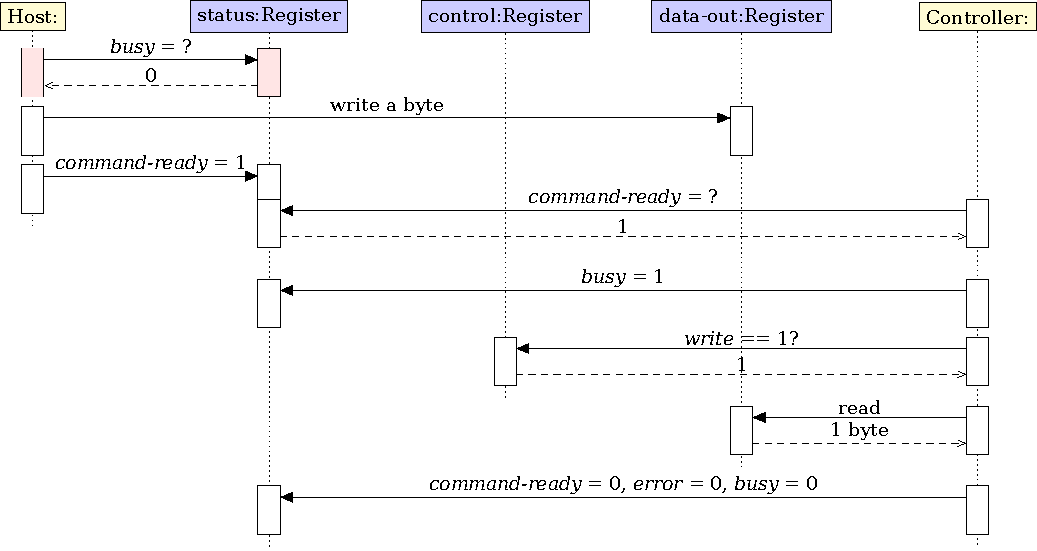
\includegraphics[width=.9\textwidth]{handshaking}
    }
  \end{center}
\end{frame}

For this example, the host writes output through a port, coordinating with the controller
by handshaking as follows\citetitle[Sec.~12.2.1, \emph{Polling}]{silberschatz11essentials}.
\begin{enumerate}
\item The host repeatedly reads the \emph{busy} bit until that bit becomes clear.
\item The host sets the \emph{write} bit in the command register and writes a byte into
  the \emph{data-out} register.
\item The host sets the \emph{command-ready} bit.
\item When the controller notices that the \emph{command-ready} bit is set, it sets the
  \emph{busy} bit.
\item The controller reads the command register and sees the \texttt{write} command.  It
  reads the \emph{data-out} register to get the byte and does the I/O to the device.
\item The controller clears the \emph{command-ready} bit, clears the \emph{error} bit in
  the status register to indicate that the device I/O succeeded, and clears the
  \emph{busy} bit to indicate that it is finished.
\end{enumerate}
This loop is repeated for each byte.

\begin{frame}{Example}{Steps in printing a string}
  \begin{center}
    \mode<beamer>{
      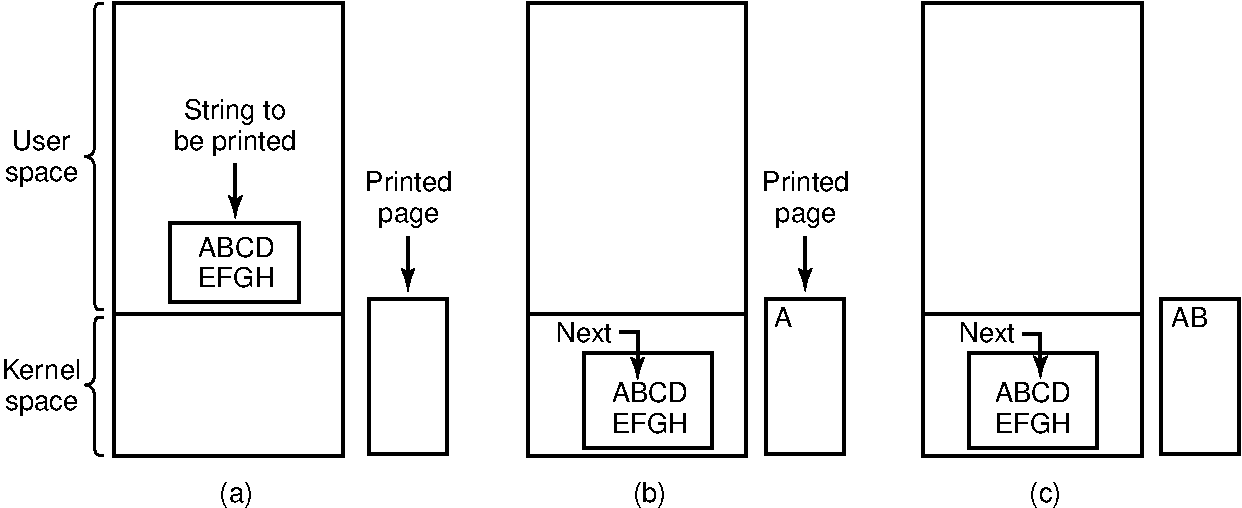
\includegraphics[width=\textwidth]{pio}
    } \mode<article>{
      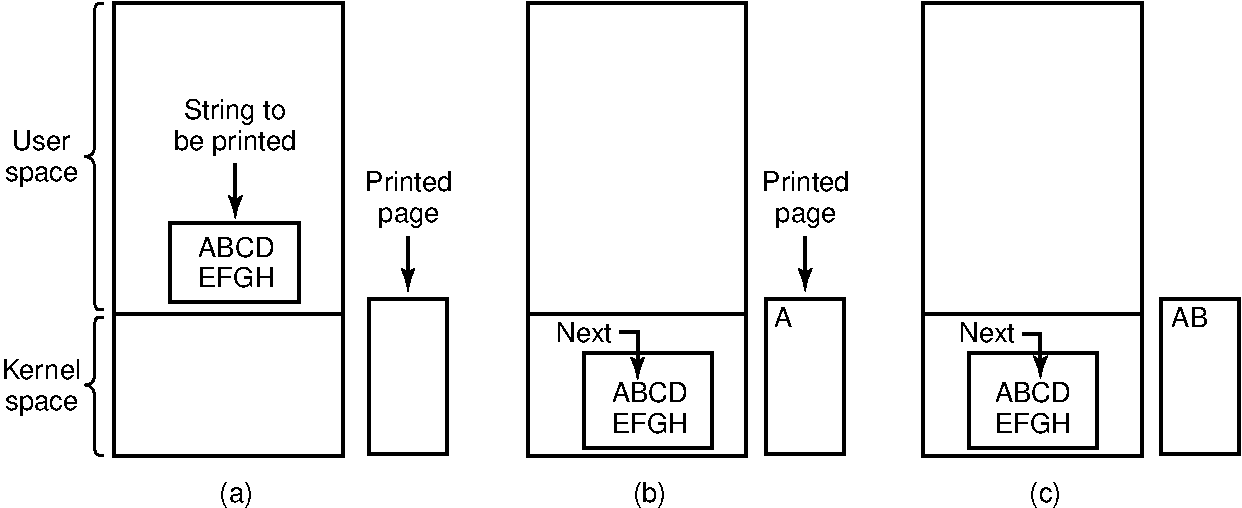
\includegraphics[width=.6\textwidth]{pio}
    }
  \end{center}
  \begin{center}
    \mode<beamer>{
      \includegraphics[width=\textwidth]{print-str}
    } \mode<article>{
      \includegraphics[width=.6\textwidth]{print-str}
    }
  \end{center}
\end{frame}

See also: \citetitle[Sec.~5.2.2, \emph{Programmed I/O}]{tanenbaum2008modern}.

\subsection{Interrupt-Driven I/O}

\begin{frame}{Pulling Is Inefficient}
  \begin{block}{A better way}
    \begin{description}
    \item[Interrupt] The controller notifies the CPU when the device is ready for service.
    \end{description}
  \end{block}
  \begin{center}
    \mode<beamer>{
      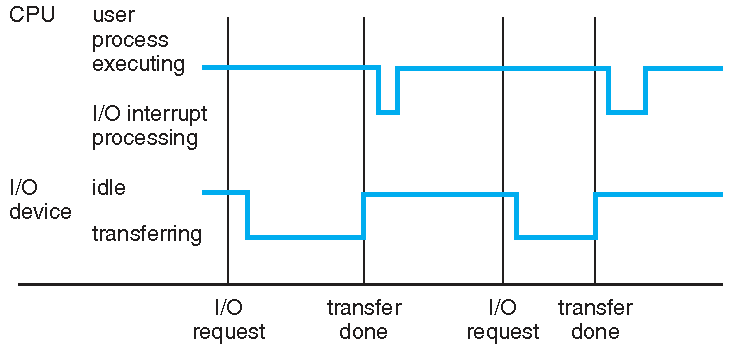
\includegraphics[width=.9\textwidth]{ir-timeline}
    } \mode<article>{
      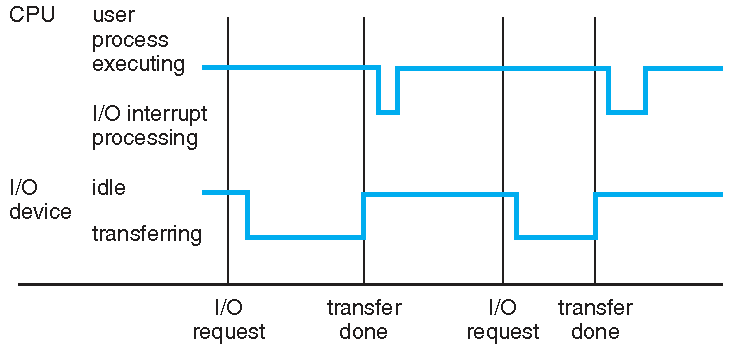
\includegraphics[width=.5\textwidth]{ir-timeline}
    }
  \end{center}
\end{frame}

See also: \citetitle[Sec.~12.2.2, \emph{Interrupts}]{silberschatz11essentials}.

\begin{frame}{Example}{Writing a string to the printer using interrupt-driven I/O}
  \begin{block}{When the print system call is made...}
    \begin{center}
      \mode<beamer>{
        \includegraphics[width=.7\textwidth]{print-str-2}
      } \mode<article>{
        \includegraphics[width=.5\textwidth]{print-str-2}
      }
    \end{center}
  \end{block}
  \begin{block}{Interrupt service procedure for the printer}
    \begin{center}
      \mode<beamer>{
        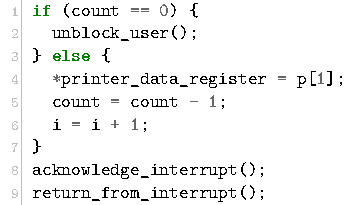
\includegraphics[width=.6\textwidth]{print-str-3}
      } \mode<article>{
        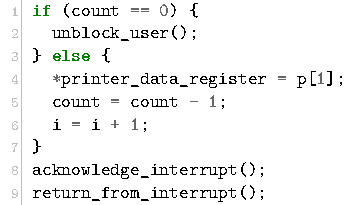
\includegraphics[width=.4\textwidth]{print-str-3}
      }
    \end{center}
  \end{block}
\end{frame}

See also: \citetitle[Sec.~5.2.3, \emph{Interrupt-Driven I/O}]{tanenbaum2008modern}.

\subsection{Direct Memory Access (DMA)}

\begin{frame}{Direct Memory Access (DMA)}
  \begin{description}
  \item[Programmed I/O (PIO)] tying up the CPU full time until all the I/O is done (busy waiting)
    % The CPU requests data from an I/O controller one byte at a
    % time. For large transfer work, such as disk I/O, PIO is wasteful.
  \item[Interrupt-Driven I/O] an interrupt occurs on every charcater (wastes CPU time)
  \item[Direct Memory Access (DMA)] Uses a special-purpose processor (DMA controller) to
    work with the I/O controller
  \end{description}  
\end{frame}

\begin{frame}{Example}{Printing a string using DMA}
  In essence, DMA is programmed I/O, only with the DMA controller doing all the work,
  instead of the main CPU.

  \begin{block}{When the print system call is made...}
    \begin{center}
      \mode<beamer>{
        \includegraphics[width=.8\textwidth]{print-str-dma-1}
      } \mode<article>{
        \includegraphics[width=.5\textwidth]{print-str-dma-1}
      }
    \end{center}
  \end{block}
  \begin{block}{Interrupt service procedure}
    \begin{center}
      \mode<beamer>{
        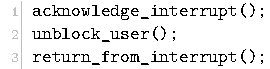
\includegraphics[width=.6\textwidth]{print-str-dma-2}
      } \mode<article>{
        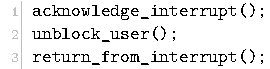
\includegraphics[width=.3\textwidth]{print-str-dma-2}
      }
    \end{center}
  \end{block}
  The big win with DMA is reducing the number of interrupts from one per character to
  one per buffer printed.
\end{frame}

The operating system can only use DMA if the hardware has a DMA controller, which most
systems do. Sometimes this controller is integrated into disk controllers and other
controllers, but such a design requires a separate DMA controller for each device. More
commonly, a single DMA controller is available (e.g., on the parentboard) for regulating
transfers to multiple devices, often concurrently\citetitle[Sec.~5.1.4, \emph{Direct Memory
  Access (DMA)}]{tanenbaum2008modern}.

\begin{frame}{DMA Handshaking Example}{Read from disk}
  \begin{center}
    \mode<beamer>{
      \includegraphics[width=\textwidth]{dma-handshaking}
    } \mode<article>{
      \includegraphics[width=.6\textwidth]{dma-handshaking}
    }
  \end{center}
\end{frame}

\begin{frame}%{The DMA Controller}
  \begin{block}{The DMA controller}
    \begin{itemize}
    \item has access to the system bus independent of the CPU
    \item contains several registers that can be written and read by the CPU. These
      includes
      \begin{itemize}
      \item a memory address register
      \item a byte count register
      \item one or more control registers
        \begin{itemize}
        \item specify the I/O port to use
        \item the direction of the transfer (read/write)
        \item the transfer unit (byte/word)
        \item the number of bytes to transfer in one burst.
        \end{itemize}
      \end{itemize}
    \end{itemize}
  \end{block}
\end{frame}

\begin{frame}%{Direct Memory Access (DMA)}
  \label{fig:dma}
  \centering \mode<beamer>{
    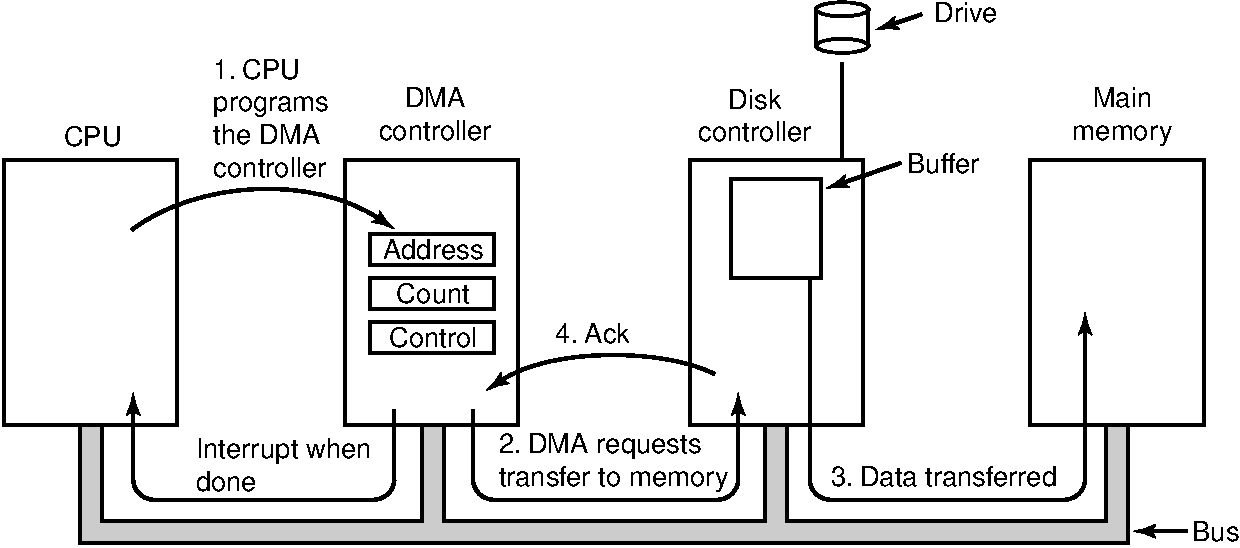
\includegraphics[width=\textwidth]{dma}
  } \mode<article>{
    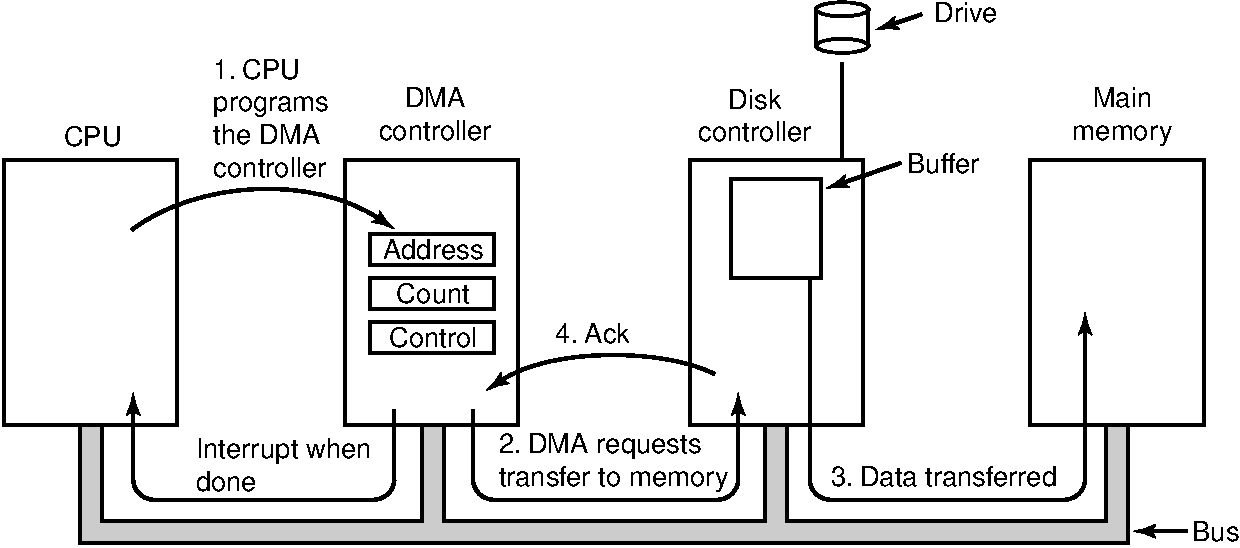
\includegraphics[width=.7\textwidth]{dma}
  }
\end{frame}

When DMA is used, ..., first the CPU programs the DMA controller by setting its registers
so it knows what to transfer where (step 1 in Fig~\ref{fig:dma}). It also issues a command
to the disk controller telling it to read data from the disk into its internal buffer and
verify the checksum. When valid data are in the disk controller's buffer, DMA can
begin\citetitle[Sec.~5.1.4, \emph{Direct Memory Access (DMA)}]{tanenbaum2008modern}.

The DMA controller initiates the transfer by issuing a read request over the bus to the
disk controller (step 2). This read request looks like any other read request, and the
disk controller does not know or care whether it came from the CPU or from a DMA
controller. Typically, the memory address to write to is on the bus' address lines so when
the disk controller fetches the next word from its internal buffer, it knows where to
write it. The write to memory is another standard bus cycle (step 3). When the write is
complete, the disk controller sends an acknowledgement signal to the DMA controller, also
over the bus (step 4). The DMA controller then increments the memory address to use and
decrements the byte count. If the byte count is still greater than 0, steps 2 through 4
are repeated until the count reaches 0. At that time, the DMA controller interrupts the
CPU to let it know that the transfer is now complete. When the operating system starts up,
it does not have to copy the disk block to memory; it is already there.


%\section{Principles of I/O Software}

\section{I/O Software Layers}

\begin{frame}{I/O Software Layers}
  \begin{center}
    \mode<beamer>{
      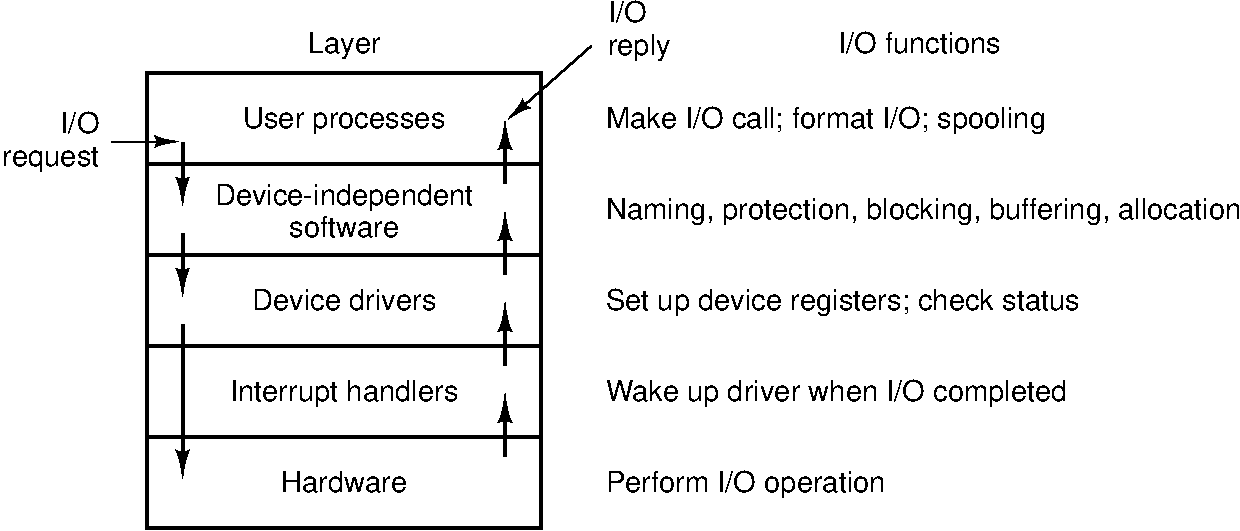
\includegraphics[width=\textwidth]{io-layers2}
    } \mode<article>{
      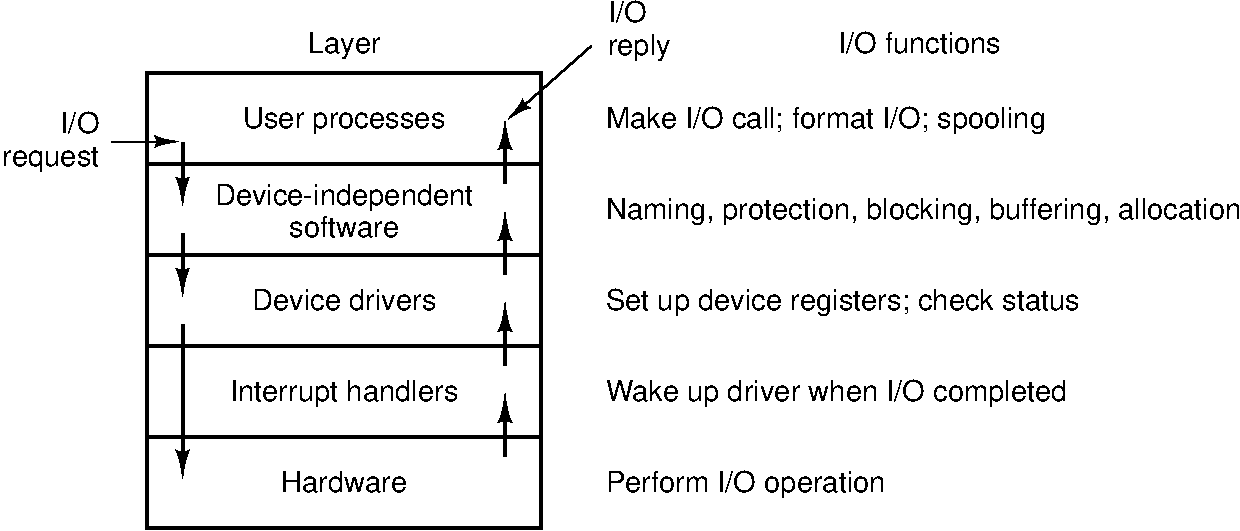
\includegraphics[width=.6\textwidth]{io-layers2}
    }
  \end{center}
\end{frame}

\subsection{Interrupt Handlers}

\begin{frame}{Interrupt Handlers}
  \begin{center}
    \mode<beamer>{
      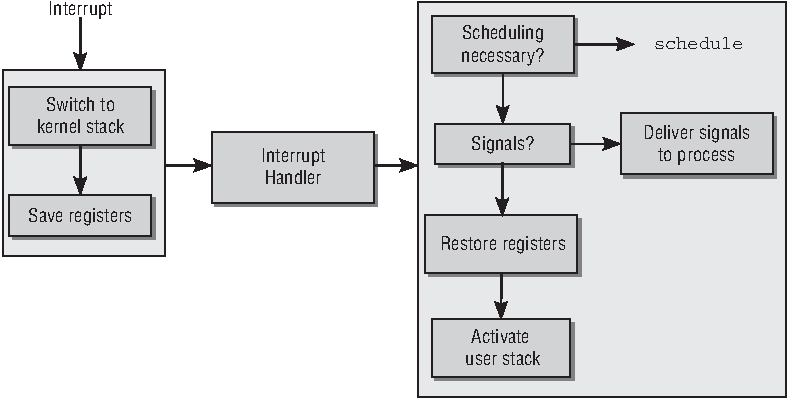
\includegraphics[width=\textwidth]{interrupt-handling}
    } \mode<article>{
      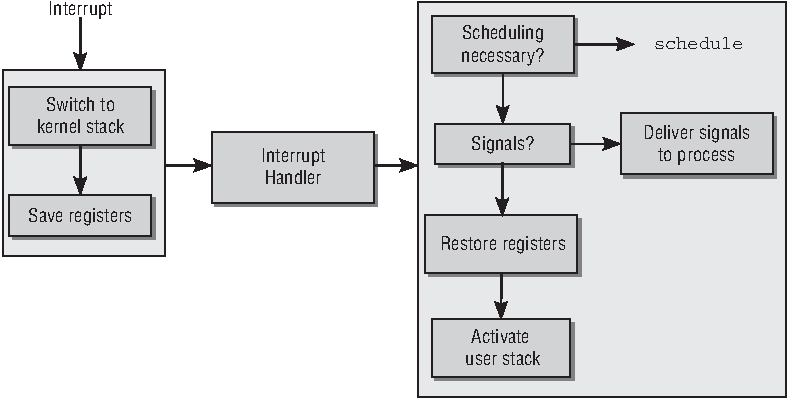
\includegraphics[width=.7\textwidth]{interrupt-handling}
    }
  \end{center}
\end{frame}

See also:
\begin{itemize}
\item \citetitle[Sec.~14.1.3, \emph{Processing Interrupts}]{mauerer2008professional}.
\item \citetitle[Sec.~5.3.1, \emph{Interrupt Handlers}]{tanenbaum2008modern}.
\end{itemize}

\subsection{Device Drivers}

\begin{frame}{Device Drivers}
  \begin{center}
    \mode<beamer>{
      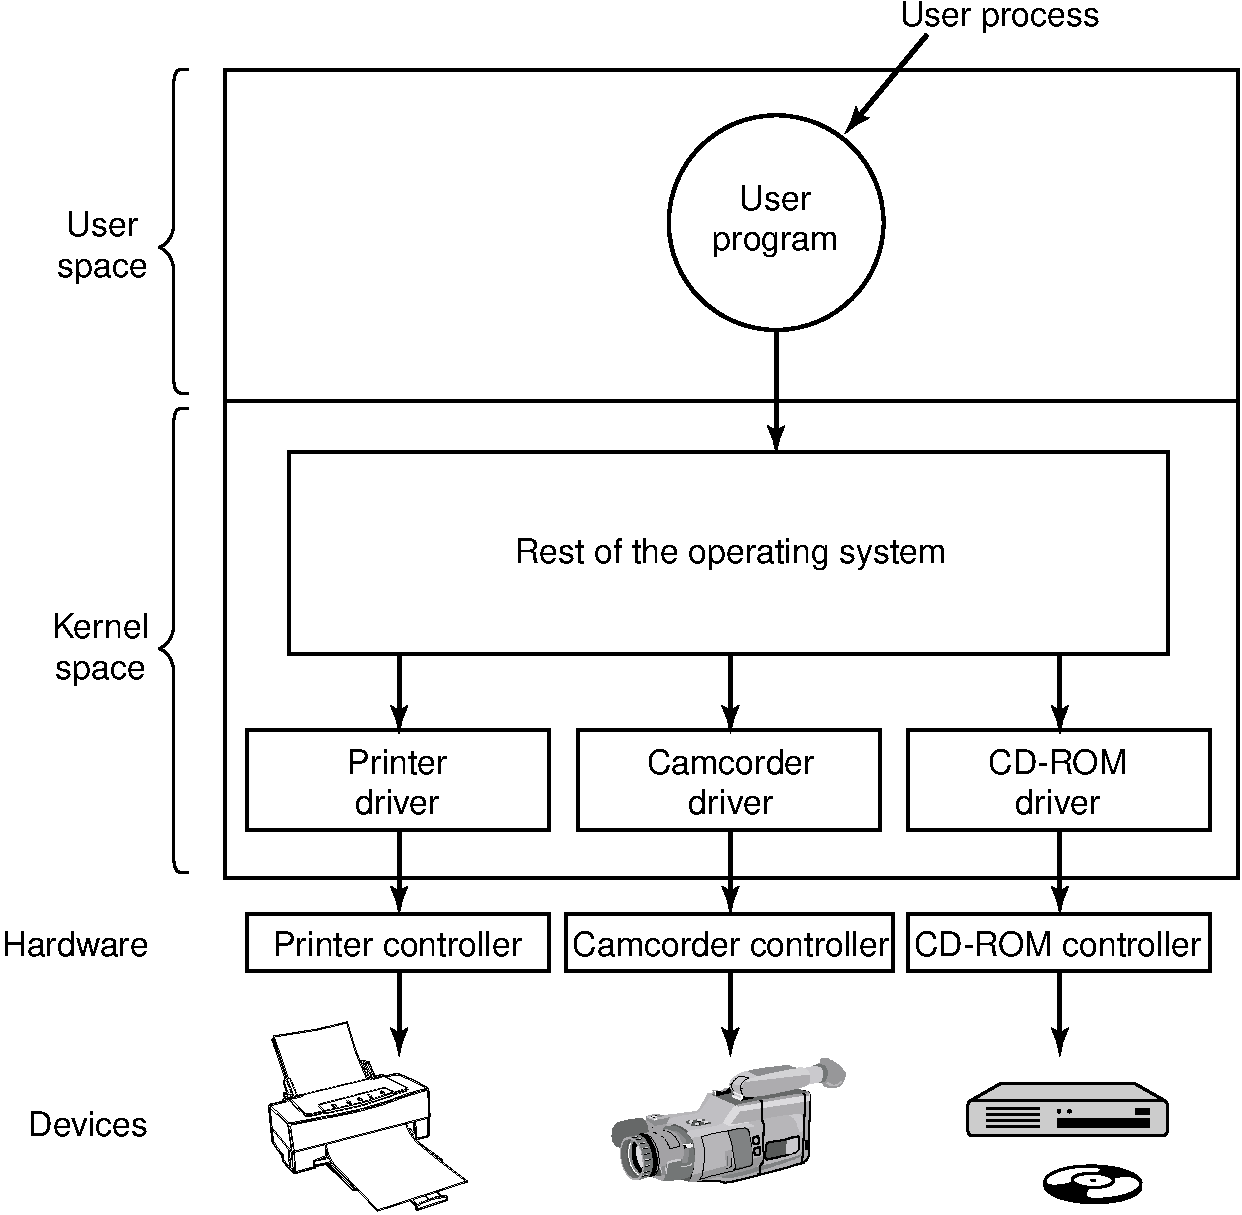
\includegraphics[width=.8\textwidth]{drivers}
    } \mode<article>{
      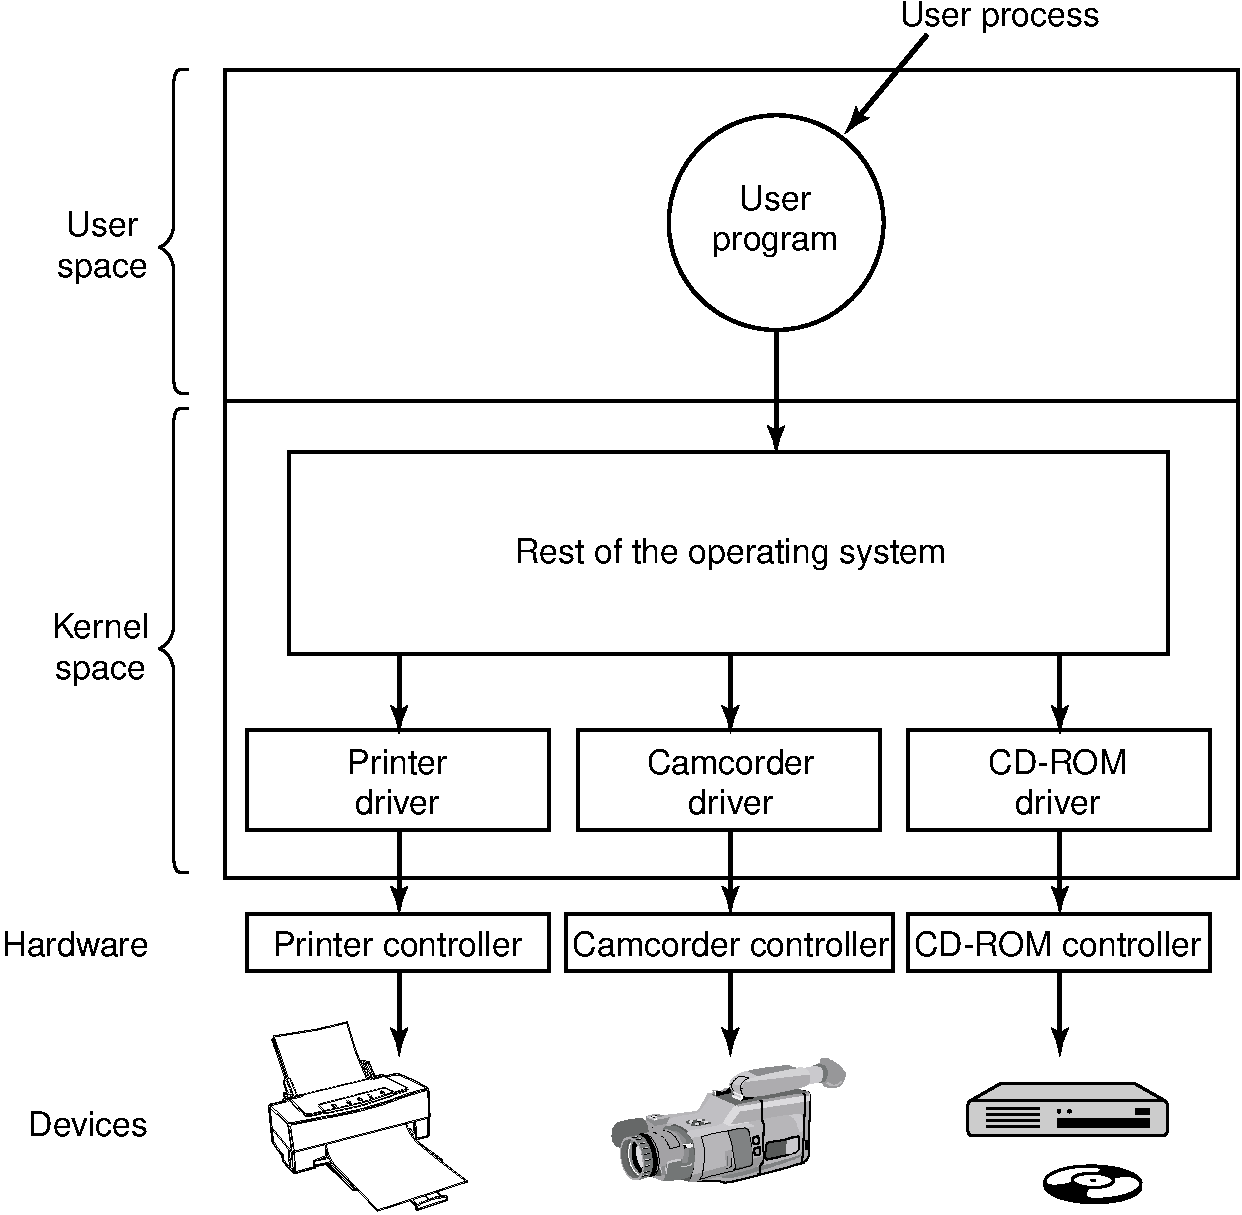
\includegraphics[width=.5\textwidth]{drivers}
    }
  \end{center}
\end{frame}

See also: \citetitle[Sec.~5.3.2, \emph{Device Drivers}]{tanenbaum2008modern}.

\subsection{Device-Independent I/O Software}

\begin{frame}{Device-Independent I/O Software}
  \begin{block}{Functions}
    \begin{itemize}
    \item Uniform interfacing for device drivers
    \item Buffering
    \item Error reporting
    \item Allocating and releasing dedicated devices
    \item Providing a device-independent block size
    \end{itemize}
  \end{block}
\end{frame}

See also: \citetitle[Sec.~5.3.3, \emph{Device-Independent I/O Software}]{tanenbaum2008modern}.

\begin{frame}{Uniform Interfacing for Device Drivers}
  \begin{center}
    \mode<beamer>{
      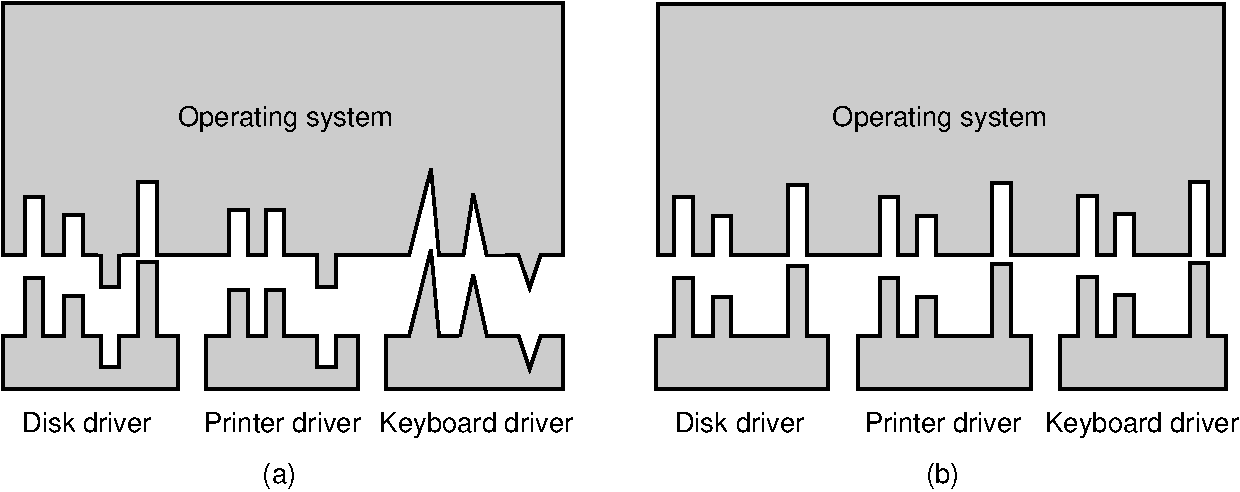
\includegraphics[width=\textwidth]{uniform-iface}
    } \mode<article>{
      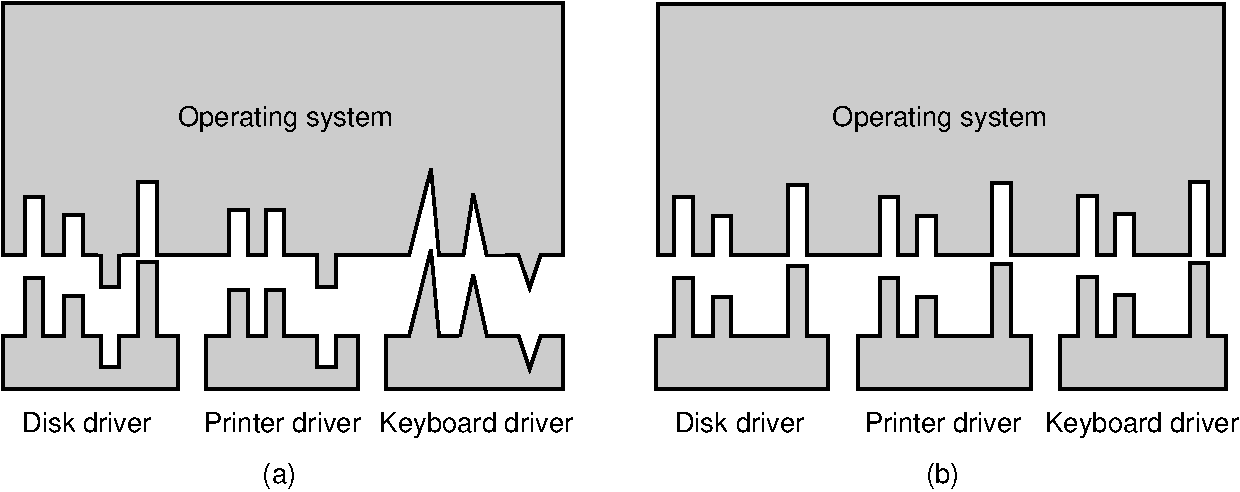
\includegraphics[width=.6\textwidth]{uniform-iface}
    }
  \end{center}
\end{frame}

\begin{frame}{Buffering}
  \begin{center}
    \mode<beamer>{
      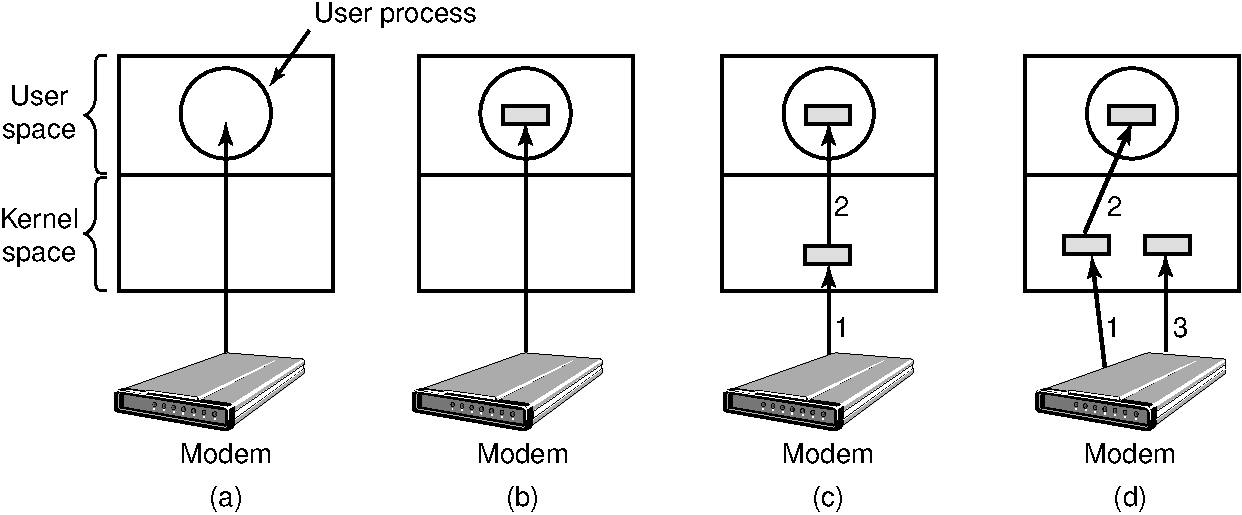
\includegraphics[width=\textwidth]{buffering}
    } \mode<article>{
      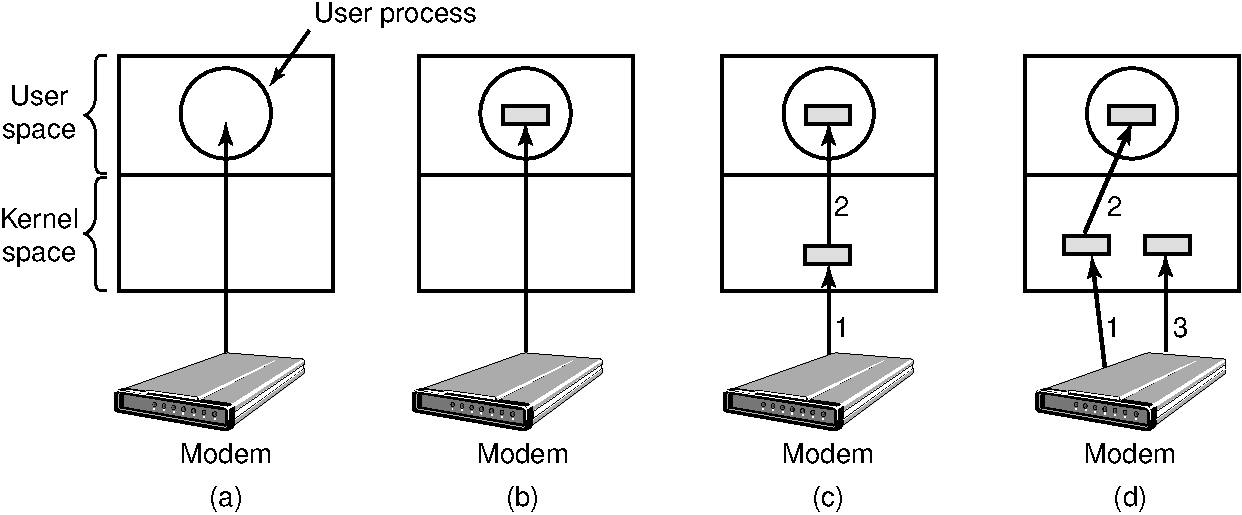
\includegraphics[width=.6\textwidth]{buffering}
    }
  \end{center}
\end{frame}

\subsection{User-Space I/O Software}

\begin{frame}{User-Space I/O Software}
  \begin{block}{Examples:}
    \begin{itemize}
    \item stdio.h, printf(), scanf()...
    \item spooling(printing, USENET news...)
    \end{itemize}
  \end{block}  
\end{frame}

See also: \citetitle[Sec.~5.3.4, \emph{User-Space I/O Software}]{tanenbaum2008modern}.

\section{Disks}

\begin{frame}{Disk}
  \begin{center}
    \mode<beamer>{
      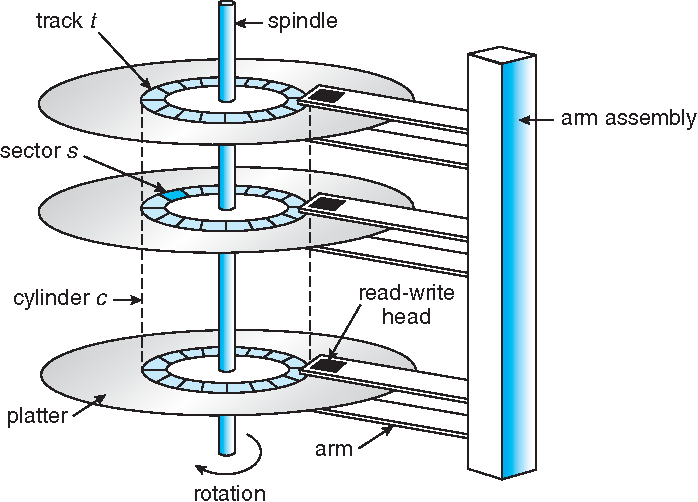
\includegraphics[width=.8\textwidth]{disk}
    } \mode<article>{
      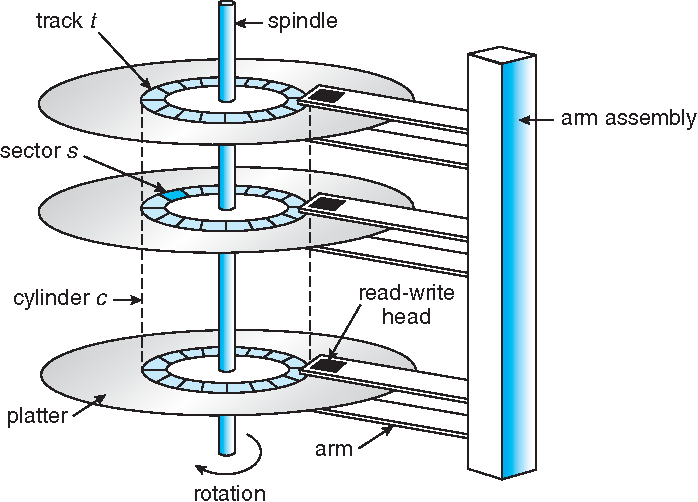
\includegraphics[width=.5\textwidth]{disk}
    }
  \end{center}
\end{frame}

A read-write head “flies” just above each surface of every platter. The heads are attached
to a \Navy{disk arm} that moves all the heads as a unit. The surface of a platter is
logically divided into circular \Navy{tracks}, which are subdivided into
\Navy{sectors}. The set of tracks that are at one arm position makes up a \Navy{cylinder}.
There may be thousands of concentric cylinders in a disk drive, and each track may contain
hundreds of sectors. The storage capacity of common disk drives is measured in
gigabytes\citetitle[Sec.~11.1.1, \emph{Magnetic Disks}]{silberschatz11essentials}.

When the disk is in use, a drive motor spins it at high speed. Most drives rotate 60 to
200 times per second. Disk speed has two parts. The \Navy{transfer rate} is the rate at
which data flow between the drive and the computer. The \Navy{positioning time}, sometimes
called the \Navy{random-access time}, consists of the time necessary to move the disk arm to
the desired cylinder, called the \Navy{seek time}, and the time necessary for the desired
sector to rotate to the disk head, called the \Navy{rotational latency}. Typical disks can
transfer several megabytes of data per second, and they have seek times and rotational
latencies of several milliseconds.

...

A disk drive is attached to a computer by a set of wires called an \Navy{I/O bus}. Several
kinds of buses are available, including enhanced integrated drive electronics
(\Navy{EIDE}), advanced technology attachment (\Navy{ATA}), serial ATA (\Navy{SATA}),
universal serial bus (\Navy{USB}), fiber channel (\Navy{FC}), and small computer-systems
interface (\Navy{SCSI}) buses. The data transfers on a bus are carried out by special
electronic processors called \Navy{controllers}. The \Navy{host controller} is the
controller at the computer end of the bus. A \Navy{disk controller} is built into each
disk drive. To perform a disk I/O operation, the computer places a command into the host
controller, typically using memory-mapped I/O ports, as described in Section 8.7.3. The
host controller then sends the command via messages to the disk controller, and the disk
controller operates the disk-drive hardware to carry out the command. Disk controllers
usually have a built-in cache. Data transfer at the disk drive happens between the cache
and the disk surface, and data transfer to the host, at fast electronic speeds, occurs
between the cache and the host controller.

\subsection{Disk Scheduling}

\begin{frame}{Disk Scheduling}{First Come First Serve (FCFS)}
  \begin{center}
    \mode<beamer>{
      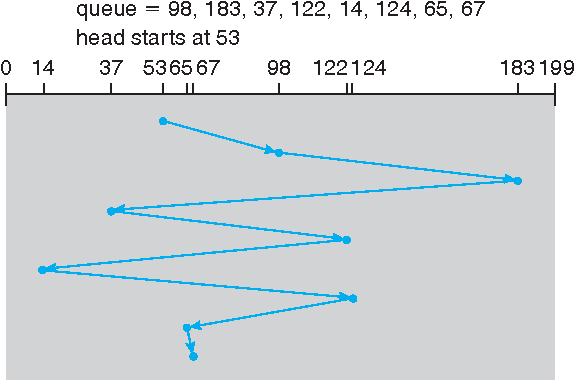
\includegraphics[width=.8\textwidth]{disk-sched-fcfs}
    } \mode<article>{
      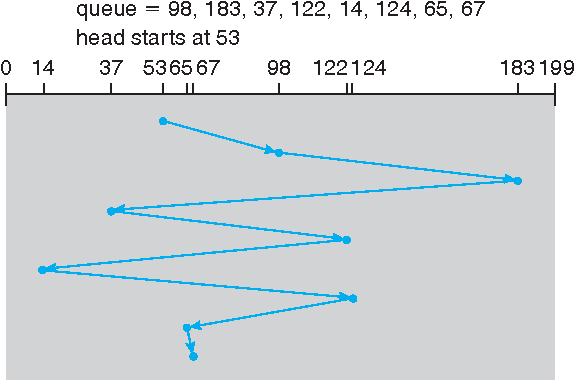
\includegraphics[width=.5\textwidth]{disk-sched-fcfs}
    }
  \end{center}
\end{frame}

If the disk head is initially at cylinder 53, it will first move from 53 to 98, then to
183, 37, 122, 14, 124, 65, and finally to 67, for a total head movement of 640
cylinders. The wild swing from 122 to 14 and then back to 124 illustrates the problem with
this schedule. If the requests for cylinders 37 and 14 could be serviced together, before
or after the requests for 122 and 124, the total head movement could be decreased
substantially, and performance could be thereby improved\citetitle[Sec.~11.4.1, \emph{FCFS
  Scheduling}]{silberschatz11essentials}.

\begin{frame}{Disk Scheduling}{Shortest Seek Time First (SSTF)}
  \begin{center}
    \mode<beamer>{
      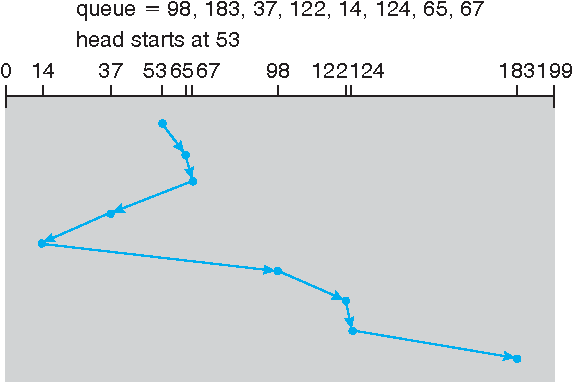
\includegraphics[width=.8\textwidth]{disk-sched-sstf}
    } \mode<article>{
      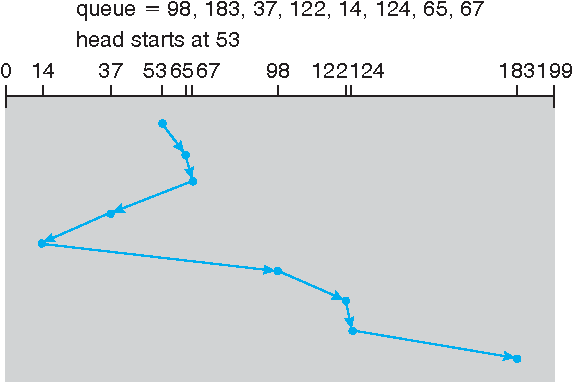
\includegraphics[width=.5\textwidth]{disk-sched-sstf}
    }
  \end{center}
\end{frame}

For our example request queue, the closest request to the initial head position (53) is at
cylinder 65. Once we are at cylinder 65, the next closest request is at cylinder 67. From
there, the request at cylinder 37 is closer than the one at 98, so 37 is served
next. Continuing, we service the request at cylinder 14, then 98, 122, 124, and finally
183. This scheduling method results in a total head movement of only 236 cylinders—little
more than one-third of the distance needed for FCFS scheduling of this request
queue. Clearly, this algorithm gives a substantial improvement in
performance\citetitle[Sec.~11.4.2, \emph{SSTF Scheduling}]{silberschatz11essentials}.

SSTF scheduling is essentially a form of shortest-job-first (SJF) scheduling; and like SJF
scheduling, \emph{it may cause starvation of some requests}. Remember that requests may
arrive at any time. Suppose that we have two requests in the queue, for cylinders 14 and
186, and while the request from 14 is being serviced, a new request near 14 arrives. This
new request will be serviced next, making the request at 186 wait. While this request is
being serviced, another request close to 14 could arrive. In theory, a continual stream of
requests near one another could cause the request for cylinder 186 to wait indefinitely.
This scenario becomes increasingly likely as the pending-request queue grows longer.

Although the SSTF algorithm is a substantial improvement over the FCFS algorithm, \emph{it
  is not optimal}. In the example, we can do better by moving the head from 53 to 37, even
though the latter is not closest, and then to 14, before turning around to service 65, 67,
98, 122, 124, and 183. This strategy reduces the total head movement to 208 cylinders.

\begin{frame}{Disk Scheduling}{SCAN Scheduling}
  \begin{center}
    \mode<beamer>{
      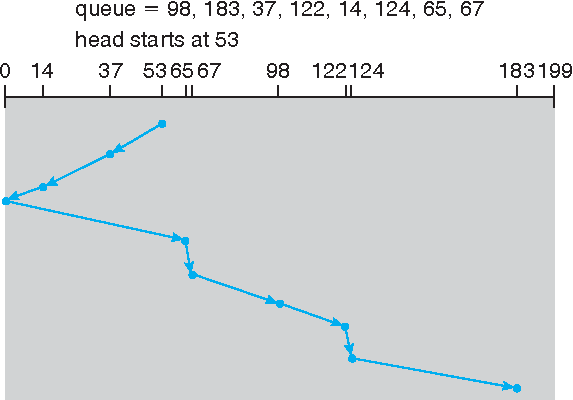
\includegraphics[width=.8\textwidth]{disk-sched-scan}
    } \mode<article>{
      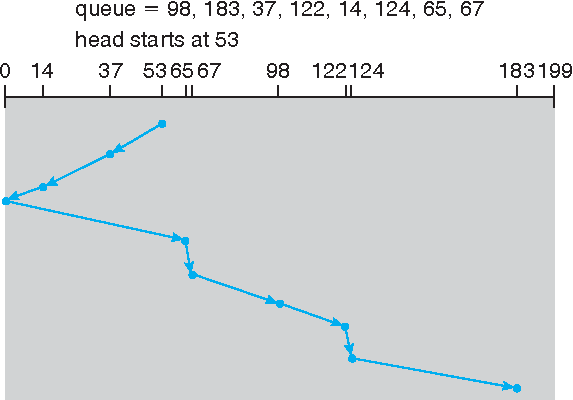
\includegraphics[width=.5\textwidth]{disk-sched-scan}
    }
  \end{center}
\end{frame}

See also: \citetitle[Sec.~11.4.3, \emph{SCAN Scheduling}]{silberschatz11essentials}.

\begin{frame}{Disk Scheduling}{Circular SCAN (C-SCAN) Scheduling}
  \begin{center}
    \mode<beamer>{
      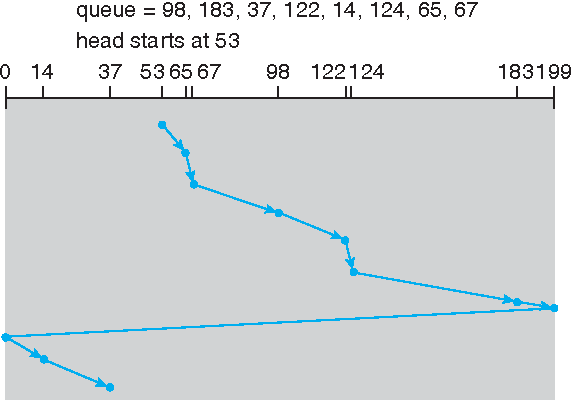
\includegraphics[width=.8\textwidth]{disk-sched-cscan}
    } \mode<article>{
      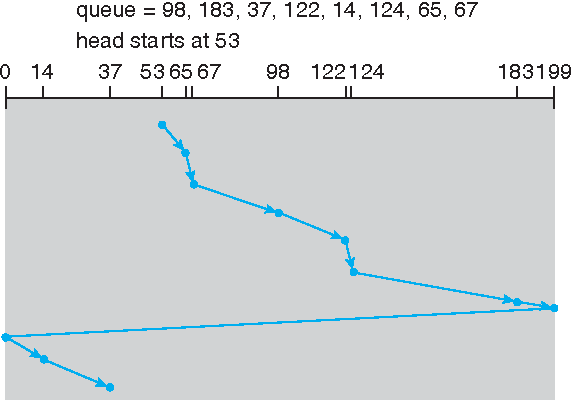
\includegraphics[width=.5\textwidth]{disk-sched-cscan}
    }
  \end{center}
\end{frame}

See also: \citetitle[Sec.~11.4.4, \emph{C-SCAN Scheduling}]{silberschatz11essentials}.

\begin{frame}{Disk Scheduling}{C-LOOK Scheduling}
  \begin{center}
    \mode<beamer>{
      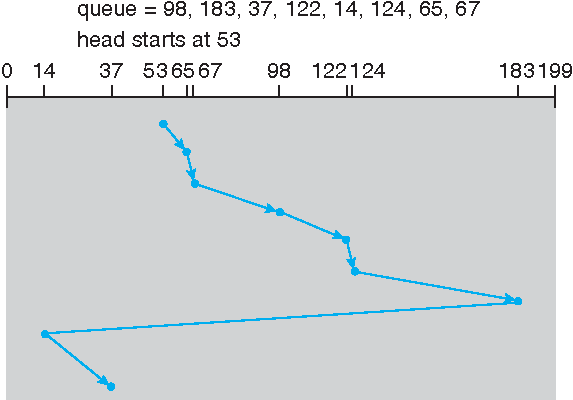
\includegraphics[width=.8\textwidth]{disk-sched-clook}
    } \mode<article>{
      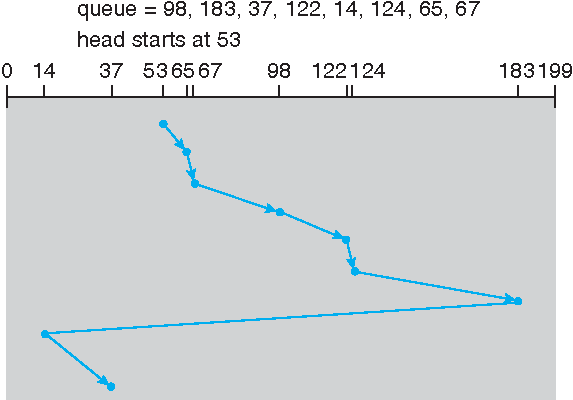
\includegraphics[width=.5\textwidth]{disk-sched-clook}
    }
  \end{center}
\end{frame}

\begin{frame}{The Best Scheduling Algorithm?}
  \begin{block}{Performance depends heavily on the number and types of requests}
    File system design can be influential
    \begin{itemize}
      % \item[e.g.] only one request in queue
    \item File-allocation method (contiguous? indexed?)
    \item Location of directories and index blocks
    \end{itemize}
  \end{block}
\end{frame}

In Linux, the \emph{deadline I/O scheduler} used in Version 2.6 works similarly to the
elevator algorithm (C-SCAN) except that it also associates a deadline with each request,
thus addressing the starvation issue. By default, the deadline for read requests is 0.5
second and that for write requests is 5 seconds. The deadline scheduler maintains a
\emph{sorted queue} of pending I/O operations ordered by sector number. However, it also
maintains two other queues --- a \emph{read queue} for read operations and a
\emph{write queue} for write operations. These two queues are ordered according to
deadline. Every I/O request is placed in both the sorted queue and either the read or the
write queue, as appropriate. Ordinarily, I/O operations occur from the sorted
queue. However, if a deadline expires for a request in either the read or the write queue,
I/O operations are scheduled from the queue containing the expired request. This policy
ensures that an I/O operation will wait no longer than its expiration
time\citetitle[Sec.~15.8.1, \emph{Block Devices}]{silberschatz11essentials}.

See also: \citetitle[Sec.~11.4.6, \emph{Selection of a Disk-Scheduling
  Algorithm}]{silberschatz11essentials}.

\subsection{RAID Structure}

\begin{frame}{RAID Structure}
  \begin{block}{Redundant Arrays of Independent/Inexpensive Disks}
    \begin{itemize}
    \item[\PackingWaste] Replace SLED with RAID
    \item[\PackingWaste] Replace the disk controller card with a RAID controller
    \item[\good] Better performance and better reliability
    \item[\good] No software changes are required to use the RAID
    \end{itemize}
  \end{block}
\end{frame}

\begin{frame}{RAID Levels}
  \begin{center}
    \mode<beamer>{
      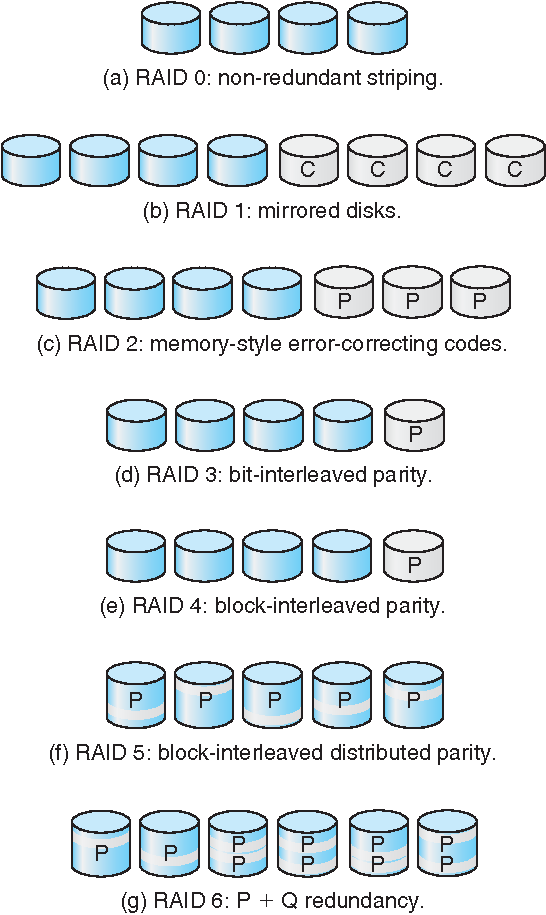
\includegraphics[height=.9\textheight]{raid-levels}
    } \mode<article>{
      \includegraphics[width=.3\textwidth]{raid-levels}
    }
  \end{center}
\end{frame}


% \section{Clocks}

% \begin{frame}{Clock Hardware}
%   \begin{itemize}
%   \item generate interrupts at known intervals
%   \end{itemize}
% \end{frame}

% \begin{frame}{Clock Software}
  
% \end{frame}


% \section{User Interfaces: Keyboard, Mouse, Monitor}


% \section{Thin Clients}


% \section{Power management}

\begin{frame}\mode<beamer>{\frametitle{References}}
  \begin{refsection}
    \nocite{wiki:disk, wiki:io}
    \printbibliography[heading=none]
  \end{refsection}
\end{frame}

\mode<all>
%%% Local Variables:
%%% mode: latex
%%% TeX-master: "os-b"
%%% End:
